\chapter{Az OSGi keretrendszerről}
\label{cha:osgi}

Az OSGi Alliance \cite{osgi} által fejlesztett OSGi (\textit{Open Services Gateway initiative}) egy Java nyelvű, dinamikus, szolgáltatás orientált komponens modell és keretrendszer, mellyel kiterjeszthető az alap Java nyelven készült programok funkcionalitása. Használatával elérhető válik egy komponens alapú fejlesztés, ahol alkalmazásokat (illetve komponenseket) távolról elérve telepíthetjük, elindíthatjuk, leállíthatjuk, frissíthetjük, vagy törölhetjük anélkül, hogy a teljes alkalmazást leállítanánk és újra elindítanánk. A standard Java-val készült alkalmazásoknál ez egy fontos hiányosság, hiszen az információs rendszerek sok területén nem engedhetőek meg akár a pillanatnyi leállások sem. A flexibilitás és újrafelhasználhatóság követelményeknek tehát nagyon jól megfelel az OSGi keretrendszer, ezért is esett rá a választás.

\section{Bundle}
\label{sec:bundle}

Az OSGi technológiát \cite{osgiintro} használó alkalmazások kisebb komponensekre (az OSGI terminológiát használva csomagokra, azaz \textit{bundle}-ökre) vannak bontva. Ezen csomagok elkészíthetőek, lefordíthatóak, telepíthetőek egymástól függetlenül, életciklusukat maga az OSGi keretrendszer felügyeli. A bundle-ök gyakorlatilag nem mások, mint a jól ismert JAR fájlok (Java osztályok, és egyéb erőforrások), azzal a különbséggel, hogy a leíró manifest állományban a szabvány által kiterjesztett módon további fejlécek találhatóak meg. Példát látunk manifest állományra a \ref{lst:manifest}.~kódrészletben.

A manifest állomány elemei:

\begin{description}
	\item[Bundle-Name] az elkészített bundle emberek számára olvasható neve
	\item[Bundle-SymbolicName] Java package név, ez azonosítja a bundle-t (az egyetlen kötelező elem)
	\item[Bundle-Description] a bundle hosszabb szöveges leírása
	\item[Bundle-ManifestVersion] a bundle által használt OSGi változat verziószáma
	\item[Bundle-Version] a bundle verziószáma
	\item[Bundle-Activator] BundleActivator interfészt implementáló bundle-ben lévő osztály, mely a bundle telepítése után elindul
	\item[Export-Package] más bundle-ök számára elérhetővé tett saját csomagok és verziószámaik listája
	\item[Import-Package] a bundle fordításához és futtatásához szükséges külső csomagok listája
	\item[Private-Package] olyan saját csomagok, amelyeket nem teszünk elérhetővé más bundle-ök számára
\end{description}

\begin{lstlisting}[label={lst:manifest}, caption=MANIFEST.MF,breaklines=true]
Bundle-Name: Hello World
Bundle-SymbolicName: org.available.helloworld
Bundle-Description: A Hello World bundle
Bundle-ManifestVersion: 2
Bundle-Version: 1.0.0
Bundle-Activator: org.available.helloworld.Activator
Export-Package: org.available.helloworld;version="1.0.0"
Import-Package: org.osgi.framework;version="1.3.0"
Private-Package: org.notavailable.helloworld
\end{lstlisting}

% section bundle (end)

A bundle-ök egy OSGi példányon belül, azonos JVM-ben futnak. Ennek vannak előnyei (teljesítmény növekedés, kisebb erőforráshasználat, interprocess kommunikációt nem szükséges használni), de hátrányai is (hozzáférési problémák), melyeket az OSGi úgy old meg, hogy minden bundle-höz saját classloader-t rendel.

\section{Service, Service Registry}
\label{sec:service}

A bundle-ök kiajánlhatnak szolgáltatásokat (\textit{service}), melyekre más bundle-ök feliratkozhatnak. Az OSGi specifikáció szerint a szolgáltatások normál Java objektumok, melyek egy adott interfészt implementálva lettek beregisztrálva az OSGi \textit{Service Registry} moduljába.

A Service Registry segítségével tudnak tehát a bundle-ök kiajánlani szolgáltatásokat, rajtuk keresztül tudják lekérdezni az elérhető szolgáltatásokat. Ha egy bundle-nek szüksége van egy másik bundle által kiajánlott szolgáltatásra, akkor az OSGi keretrendszer megteremti közöttük a kapcsolatot és a kért szolgáltatást használhatja az adott bundle.

% section service (end)

\section{Életciklus}
\label{sec:lifecycle}

\begin{figure}[htb]
\centering
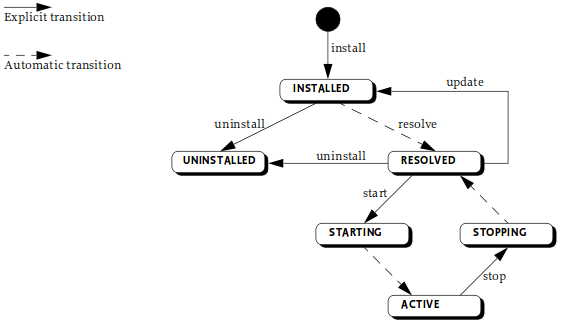
\includegraphics[scale=0.5]{img/bundle_lifecycle}
\caption{Bundle életciklus (forrás: OSGi Service Platform Release 2 \cite{osgi})}
\label{fig:bundle_lifecycle}
\end{figure}

\begin{table}[htb]
\begin{center}
\begin{tabular}{|c|c|}
\hline
\textbf{Állapot neve} & \textbf{Leírás} \\
\hline
\hline
INSTALLED   & A bundle sikeres telepítve lett. \\
\hline
RESOLVED    & A bundle-nek minden függősége ki lett elégítve. Kész az elindításra, vagy már le lett állítva. \\
\hline
STARTING    & A bundle el lett indítva, de még nincs aktiválva, .start() metódus még nem tért vissza. \\
\hline
ACTIVE      & A bundle aktiválva lett és aktív. \\
\hline
STOPPING    & A bundle le lett állítva, .stop() metódus még nem tért vissza. \\
\hline
UNINSTALLED & A bundle el lett távolítva, ez az életciklus végállapota. \\
\hline
\end{tabular}
\end{center}
\caption{\label{tab:lifecycle_states} Bundle életciklus állapotai}
\end{table}

Az OSGi keretrendszer dinamikusságát a \textit{Life-cycle} (életciklus) modul szolgáltatja, mely által a bundle-öket futásidőben lehet telepíteni, elindítani, leállítani, frissíteni, eltávolítani más hagyományos alkalmazásokkal ellentétben. A bundle-ök futtatása előtt megvizsgálja a keretrendszer a csomag futás idejű függőségeit, és ha olyan kielégítetlen függőségeket talál, melyek szükségesek a bundle futtatásához, akkor nem indítja el a komponenst.

Egy bundle életciklusának állapotai megfigyelhetőek a \ref{fig:bundle_lifecycle}.~ábrán, valamint az állapotok leírása a \ref{tab:lifecycle_states}.~táblázatban látható.

% section lifecycle (end)

% chapter osgi (end)